\subsection{Disconnect Events of RIPE Atlas Probes} \label{sec:disconnect-events}

Probes in RIPE Atlas automatically monitor the events when they are
disconnected from RIPE Atlas and when they re-connect again. Those disconnect
events give evidence about the state of a network. Frequently occurring
disconnect events might indicate an unhealthy network connection.

We analyzed the number of disconnect events for the Starlink probes in RIPE
Atlas. Figure~\ref{fig:disconnect-events-absolute} shows the number of
disconnect events per month in the time from January 2022 to July 2024.

\begin{figure}
	\centering
	\begin{subfigure}[b]{0.48\linewidth}
		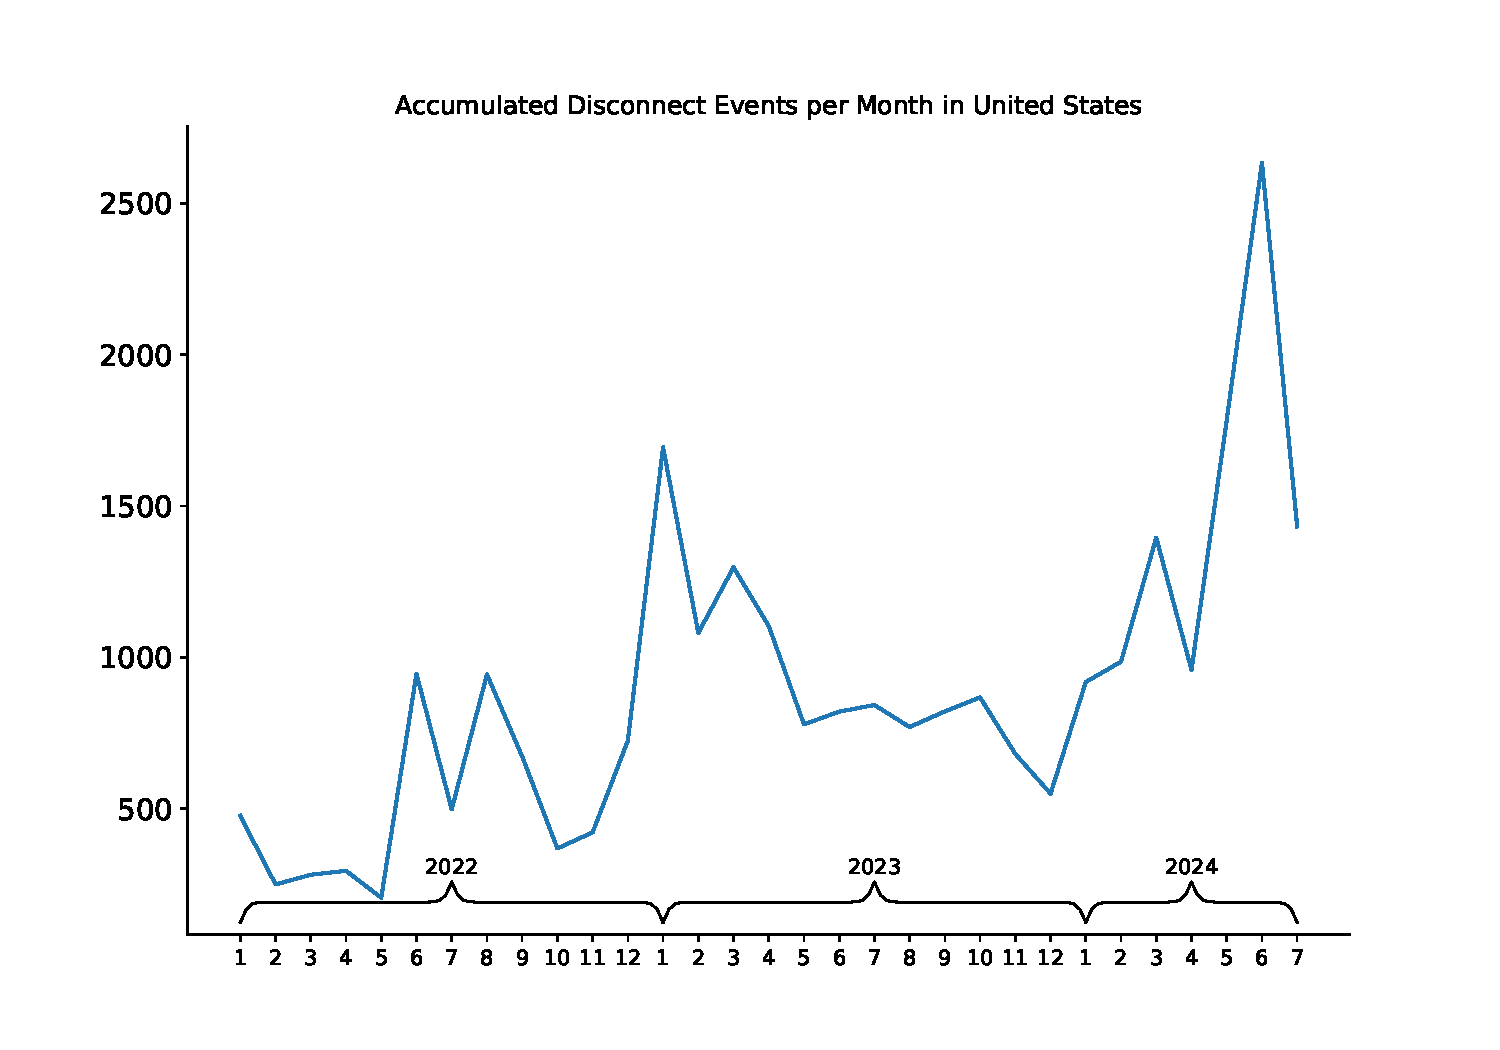
\includegraphics[width=\linewidth]{./chapters/4-results/disconnect_events/US.pdf}
		\caption{USA}
	\end{subfigure}
	\begin{subfigure}[b]{0.48\linewidth}
		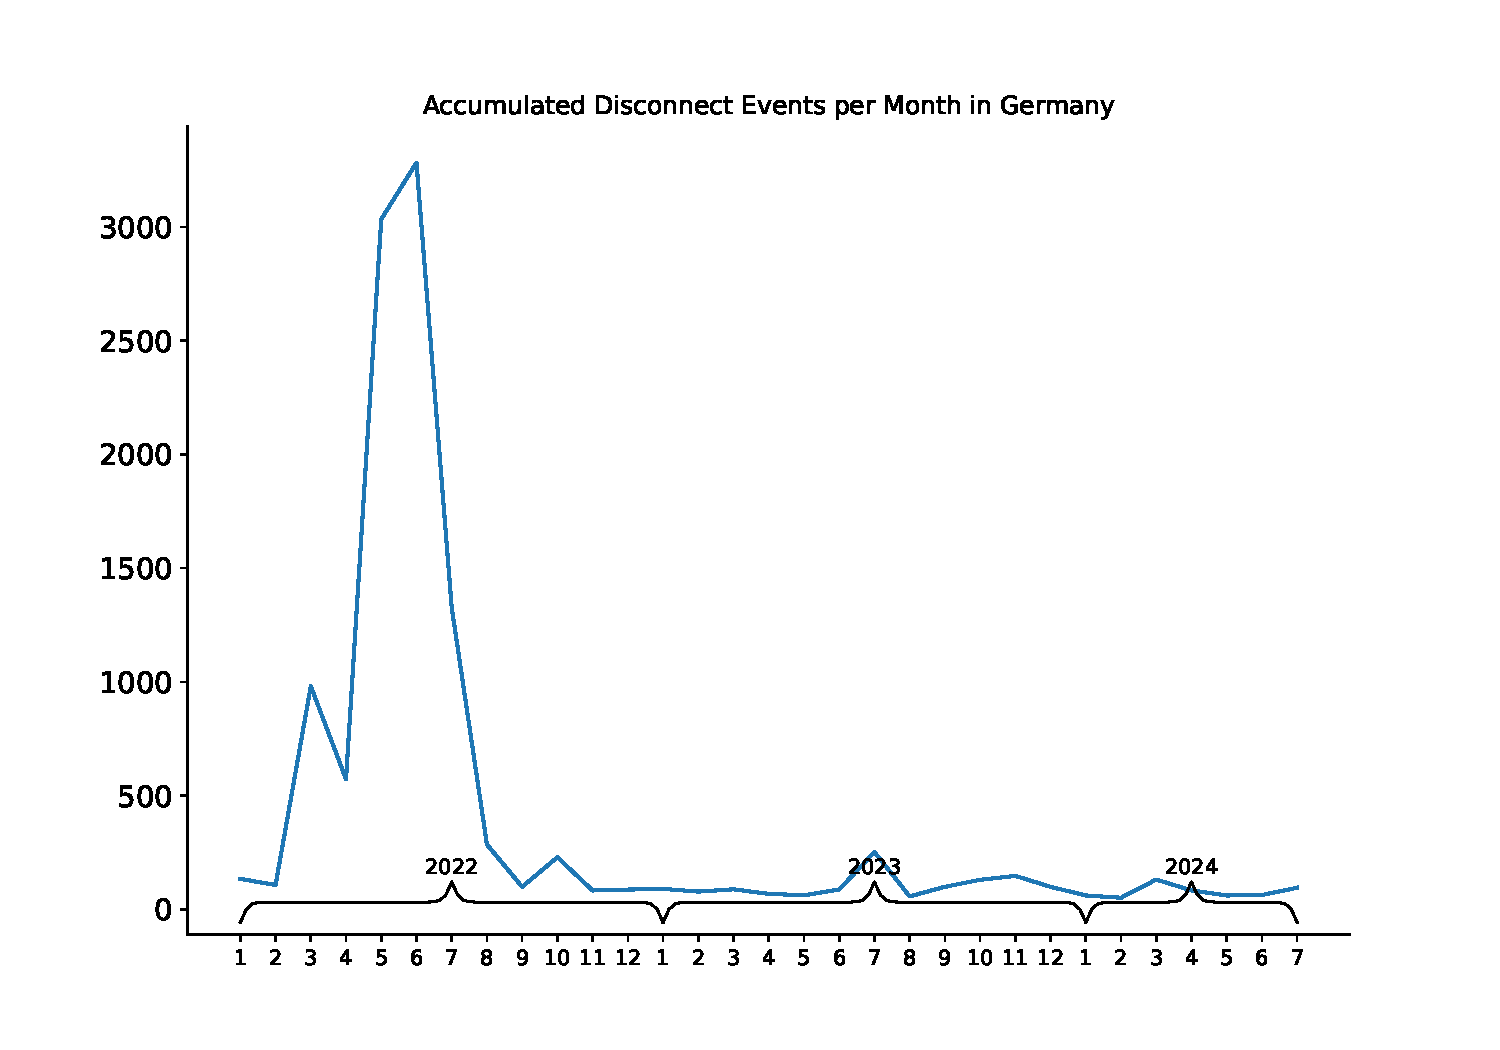
\includegraphics[width=\linewidth]{./chapters/4-results/disconnect_events/DE.pdf}
		\caption{Germany}
	\end{subfigure}
	\begin{subfigure}[b]{0.48\linewidth}
		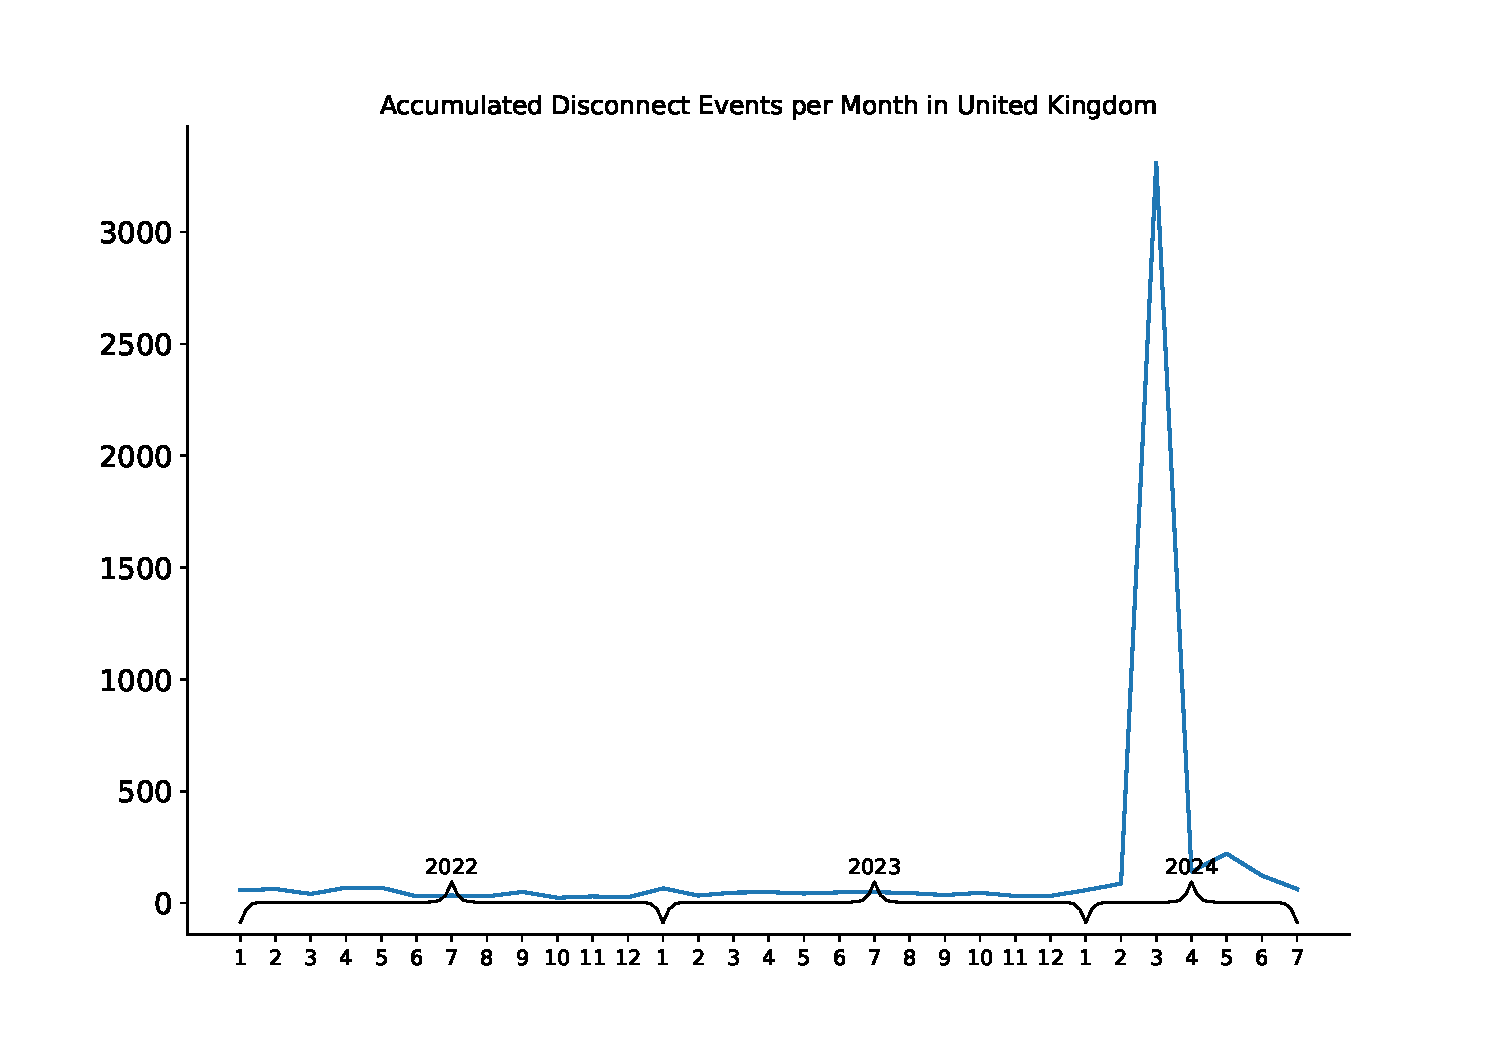
\includegraphics[width=\linewidth]{./chapters/4-results/disconnect_events/GB.pdf}
		\caption{United Kingdom}
	\end{subfigure}
	\caption{Number of Disconnect Events in the USA, Germany, and the
		United Kingdom from January 2022 to July 2024.}
	\label{fig:disconnect-events-absolute}
\end{figure}

One sees variously different patterns. While in Germany and the United Kingdom
very little disconnect events appear for the most time, the United States show
a relatively high number of disconnect events, increasing over time. The USA
experiences higher levels of disconnect events in June 2024, January 2023, and
May to August 2022. A clear pattern is not visible here. On the other side,
Germany experiences a high number of disconnect events in May to August 2022
(which also happens in the USA), while the United Kingdom does not show such a
behavior. The UK experiences a higher number of disconnect events in March
2024, but never before that. There is no clear pattern observable, when
comparing those three countries. A similar behavior was observed for other
countries.

Still, accumulating the number of disconnect events over all countries show
significant spikes. Figure~\ref{fig:disconnect-events-absolute-all-countries}
illustrates the pattern. Especially September and October 2023, the beginning
of 2024 and June 2024 show a much higher frequency. May and June 2022 have a
significant spike.

\begin{figure}
	\centering
	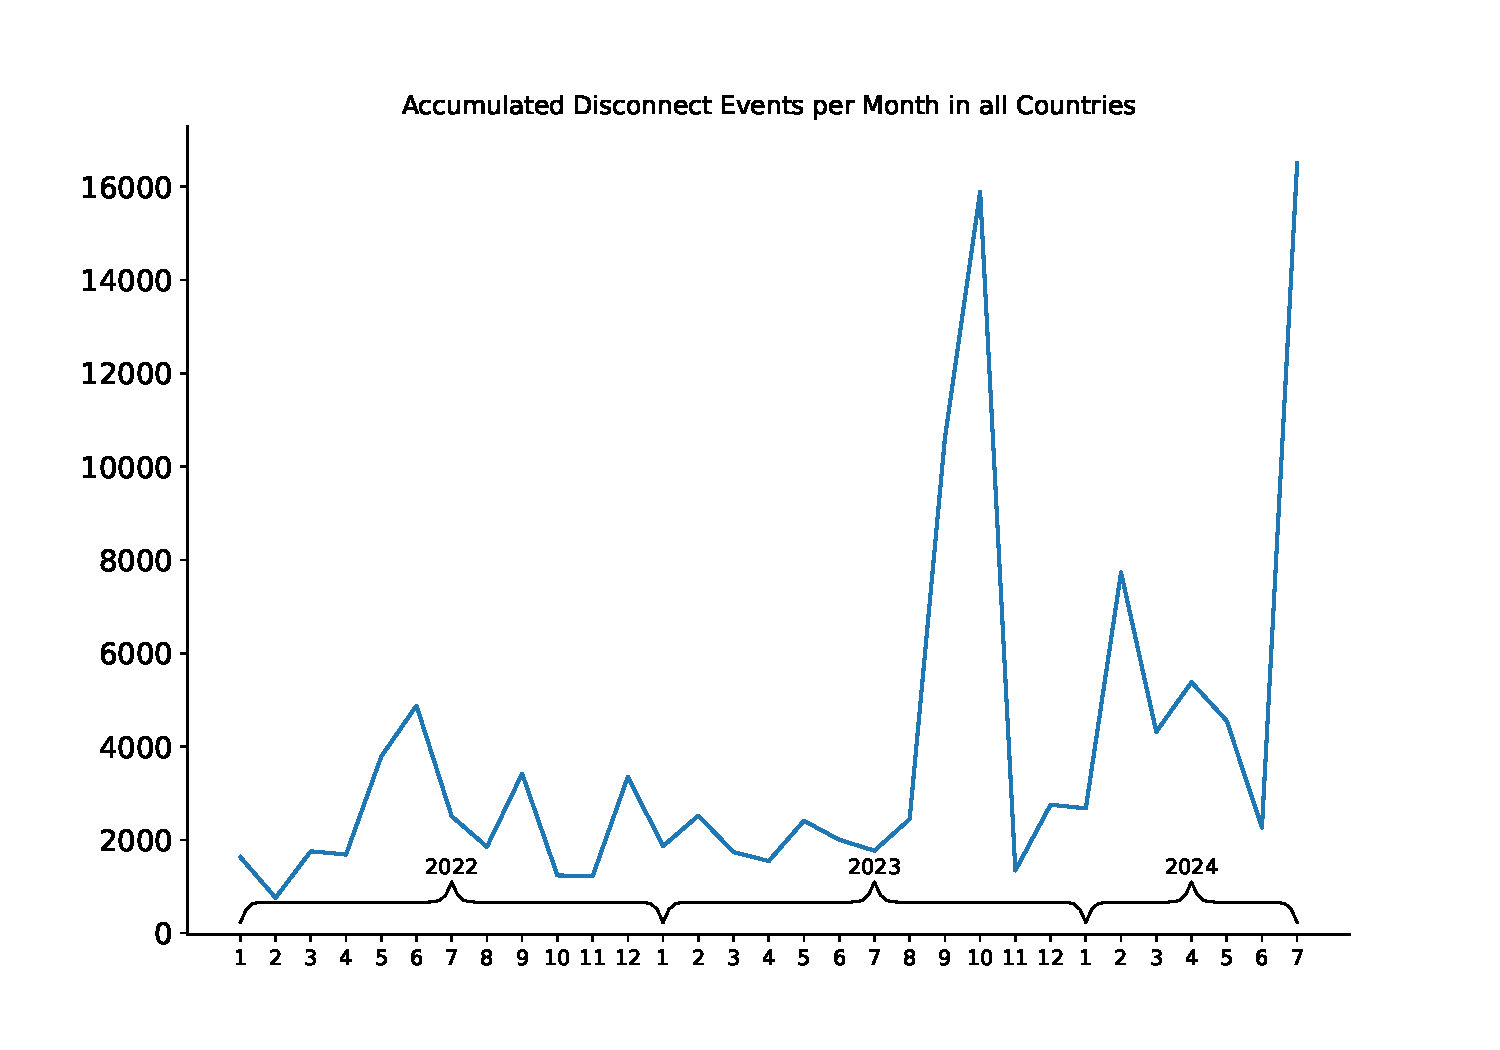
\includegraphics[width=.7\linewidth]{./chapters/4-results/disconnect_events/accumulated_disconnect_events_per_month_in_all_countries.pdf}
	\caption{Accumulated Number of Disconnect Events per Month in all
		Countries}
	\label{fig:disconnect-events-absolute-all-countries}
\end{figure}

We have to note that the data shown in
Figure~\ref{fig:disconnect-events-absolute-all-countries} does not allow making
conclusions. It holds different numbers of probes over time, so an increase in
disconnect events is expected. To draw conclusions for Starlink behavior, the
data needs to be normalized. Chapter~\ref{sec:correlation-disconnect-events}
explains this problem in more detail.

\begin{takeaway}{Usage of Disconnect Events}
	Accumulating Disconnect Events of Starlink probes seem to show a
	behavior that causes time intervals with higher occurrences. However,
	normalization is required to verify the observation. Normalization
	would be possible by using the active number of probes per time
	interval, but this was not done as it is not an easy task.
\end{takeaway}

\subsection*{Correlation of Disconnect Events with other Metrics}
\label{sec:correlation-disconnect-events}

One could correlate the occurrences of disconnect events with other metrics
(e.g., latencies and packet loss). Usually, this is done by comparing two
metrics with each other, where each metric is normalized. By normalizing, two
values of the same metric are comparable. In the case of disconnect events, the
number of disconnect events per time interval grows with the number of probes
connected. Therefore, the number of occurrences would be normalized by number
of probes connected.

However, the number of probes connected within a time interval is hard to find.
Some probes might be connected for a longer time than others dominating the
occurrences of disconnect events. Others might be connected for a very short
interval with many disconnects. Both scenarios compromise the normalization of
the disconnect event occurrences, leading to not meaningful results.\footnote{It
	might be well-possible to find a normalization method for disconnect events,
	but we did not invest in this direction.}

Therefore, we did not proceed further in correlating disconnect events with
other metrics.
